%!TEX root = pag0.tex
\chapter{Tracking and Matching tramite SIFT}
\label{chapter3}

Il tracking è l'operazione di seguire lo spostamento di un oggetto o di un insieme di punti in frame consegutivi. I punti usati per questa operazioni vengono chiamati \emph{features}. La qualità del tracking influenza in maniera molto significativa gli algoritmi che lo utilizzano. Nel codice sviluppato, il tracking viene utilizzato per stimare la posizione delle features dato il loro moto. 
Per lo studio in esame si è deciso di usare il tracking con il \emph{SIFT} acronimo di Scale-Invariant Feature Transform. Gli operatori utilizzati tradizionalmente in fotogrammetria (Forstner e Gulch 1988 ~\cite{Forstner}; Harris e Stephens 1988 ~\cite{Harry}) ricercano punti omologhi (point detector) su spigoli o discontinuità radiometriche; al contrario l’operatore SIFT ricerca i punti (keypoint) su regioni più ampie dell’immagine (region detector) superando i problemi di occlusione e deformazione prospettiche.
Questo metodo è stato sviluppato da D. G. Lowe ~\cite{Sift} e permette di rilevare i punti caratteristici di una immagine e di associargli dei descrittori basati sui gradienti delle aree dell'immagine nell'intorno delle features. Questi descrittori sono utilizzati per ricercare il punto nelle immagini successive.
I passi principali dell’algoritmo SIFT sono i seguenti:
\begin{itemize}
  \item Individuazione degli estremi locali nello scale-space: si cercano punti interessanti su tutte le scale e posizioni dell’immagine utilizzando una funzione DoG -Difference of Gaussian-. L’approccio utilizzato è quello del filtraggio in cascata (cascade filtering approach), che consente di determinare le posizioni e la scala delle features candidate ad essere punti chiave e che, in un secondo momento, vengono caratterizzate con maggior dettaglio.
  \item Localizzazione dei keypoint: per ciascun punto candidato viene costruito un modello dettagliato per determinarne posizione e scala. I punti vengono inoltre selezionati secondo misure di stabilità.
  \item Generazione delle orientazioni: per ottenere l’invarianza rotazionale, ad ogni punto chiave (keypoint) vengono associate una o più orientazioni calcolate in base ai gradienti locali dell’immagine.
  \item Generazione del descrittore: a partire dai gradienti locali dell’immagine, alla scala selezionata e nell’intorno del punto chiave, viene costruito il descrittore.
\end{itemize}
Lo scale-space è una funzione che permette di calcolare punti dell’immagine che sono invarianti a cambiamenti di scala definito come una funzione $L(x,y,\sigma)$ data dalla convoluzione in $x$ e $y$ di una funzione Gaussiana, variabile in scala, $G(x,y,\sigma)$ con l’immagine $I(x,y)$:
\begin{equation}
L(x,y,\sigma) =  G(x,y,\sigma) \otimes I(x,y)
\label{eq:surface_modeling}
\end{equation}
Ogni immagine è filtrata mediante convoluzioni di gaussiane, formando uno spazio delle \lq \lq scale \lq \lq. Per ogni scala sono quindi calcolate le differenze fra gaussiane adiacenti DoG, i cui massimi sono memorizzati come punti di interesse \emph{keypoints} ~\ref{fig:scale_gaussian}.
\begin{figure}[H]
   \centering
   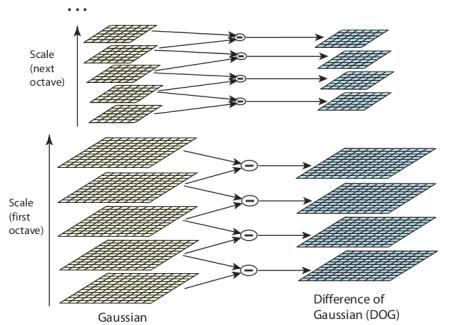
\includegraphics[width=.7\columnwidth]{sift.jpg}
   \caption{Difference of Gaussian}
   \label{fig:scale_gaussian} 
\end{figure}
Per ogni keypoint individuato è quindi definito un descrittore capace di descrivere i gradienti radiometrici nell’intorno del punto di interesse indipendentemente da rotazioni, variazioni di scala e cambiamenti di illuminazione. In base alla distanza euclidea fra questi vettori n-dimensionali è infine possibile individuare keypoints omologhi fra le immagini. Un esempio di punti di interesse estratti è mostrato in figura ~\ref{fig:keypoint}
\begin{figure}[H]
   \centering
   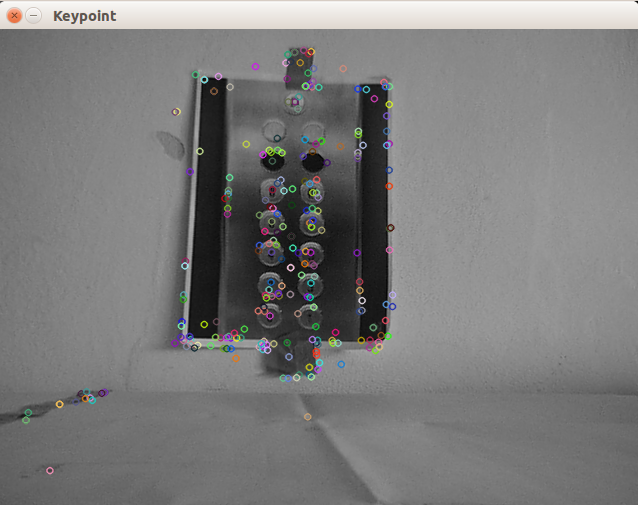
\includegraphics[width=1.\columnwidth]{keypoint.png}
   \caption{Keypoint}
   \label{fig:keypoint} 
\end{figure}
Il keypoint è quindi costituito dalle seguenti informazioni:
\begin{itemize}
\item posizione nel piano immagine
\item scala alla quale è stato rilevato il punto caratteristico
\item orientamento ossia la direzione principale del gradiente della regione nell'intorno del punto
\item descrittore che descrive in maniera univoca il punto caratteristico
\end{itemize}
Ad ogni frame vengono calcolati i keypoint e i relativi descrittori. Per ogni feature della prima immagine viene confrontato il suo descrittore con tutti i descrittori dei keypoint della seconda immagine. Il punto caratteristico con il descrittore che gli assomiglierà di più e che supera una soglia di somiglianza verrà definito come il punto corrispondente della prima immagine. In figura ~\ref{fig:matching} si può vedere un esempio di matching per il compito in esame.
\begin{figure}[H]
   \centering
   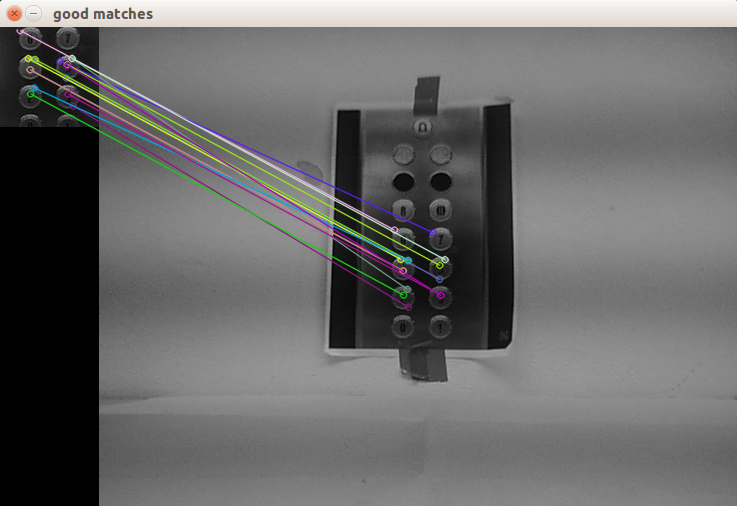
\includegraphics[width=1.\columnwidth]{match1.png}
   \caption{Match tra due frame consegutivi}
   \label{fig:matching} 
\end{figure}